%TC:group table 0 1
%TC:group tabular 1 1

\chapter{Preparation}

This chapter introduces Prolog (Section \ref{sec:prolog}) and how garbage collection techniques can be applied to it (Section \ref{sec:prolog-gc}). It also discusses web development with WebAssembly (Section \ref{sec:webdev}), before describing the tools (Section \ref{sec:tools}) and development methodology (Section \ref{sec:dev-methodology}) used in the implementation of the Prolog interpreter. Finally, a requirements analysis is performed (Section \ref{sec:requirements}) and the starting point of the project stated (Section \ref{sec:starting-point}).

\section{Prolog}

\label{sec:prolog}

Prolog is rooted in the fundamental idea that logic can be used as a programming language \cite{kowalskiPredicateLogicProgramming1974}. This section summarises the theory behind Prolog, as well as its execution model and practical implementation details.

\subsection{Clauses and Terms}

Prolog is based on \emph{first-order logic}, specifically \emph{Horn clauses}, which are of the form
$$
B \leftarrow A_1 \land \cdots \land A_n
$$
where $B$ is a positive literal (the \emph{head}) and $A_1, \ldots, A_n$ are negative literals (the \emph{body}). The key insight of Kowalski's \emph{logic programming} paradigm is that we can interpret Horn clauses as procedures of a simple programming language, written in Prolog syntax as
$$
\texttt{B :- A$_1$, $\ldots$, A$_n$.}
$$
A \emph{fact} is a Horn clause with an empty body, and a \emph{goal} is a Horn clause with an empty head.
$$
\texttt{B.} \quad \text{(fact)} \qquad\qquad\qquad \texttt{?- A$_1$, $\ldots$, A$_n$.} \quad \text{(goal)}
$$

Prolog clauses are built up from \emph{terms}, which may be
\begin{itemize}
\item \emph{atoms}, which are either \emph{constants} (e.g. \texttt{foo}, \texttt{1209}) or \emph{variables} (e.g. \texttt{X}, \texttt{Var}), or
\item \emph{compound terms}, which consist of a \emph{functor} (an atom) and a list of \emph{arguments}, which are terms themselves (e.g. \texttt{is\_even(X)}, \texttt{city(cambridge, united\_kingdom)}).
\end{itemize}

A Prolog program comprises a set of clauses and a \emph{query}, which is a goal clause. The aim of the Prolog execution is to find a \emph{substitution} (an assignment of terms to variables) that makes the query true with respect to the program.

\subsection{Most General Unification}

\emph{Unification} is the process of finding a \emph{substitution} that makes two terms equal. A substitution $\theta$ is a set of variable assignments, written $[t_1/x_1, \ldots, t_n/x_n]$, where $t_i$ are terms and $x_i$ distinct variables. A substitution is a \emph{unifier} of two terms $t_1$ and $t_2$ if $t_1\theta = t_2\theta$. The \emph{most general unifier} (MGU) $\theta$ of two terms is a unifier that is more general than any other unifier, that is, all other unifiers $\phi$ can be written as the composition of $\theta$ and another substitution $\psi$. This ensures that, if a solution exists, it will not be missed.

\paragraph{Martelli-Montanari Algorithm}

The \emph{Martelli-Montanari algorithm} is an algorithm for computing the most general unifier of two terms $t_1$ and $t_2$ \cite{martelliEfficientUnificationAlgorithm1982}. It iteratively applies rules to a set of equations, starting with $\{t_1 = t_2\}$, until no more rules can be applied, at which point the remaining set of equations is the unifier.

The rules are shown in Figure \ref{fig:martelli-montanari}. $s$ and $t$ are terms, $X$ and $Y$ are variables, $f$ and $g$ are function symbols, and $S$ is a set of equations. $\text{vars}(t)$ denotes the set of variables occurring in $t$.

\begin{figure}[H]
\begin{align*}
\{f(s_1, \ldots, s_n) = f(t_1, \ldots, t_n)\} \cup S &\rightarrow \{s_1 = t_1, \ldots, s_n = t_n\} \cup S \\
\{f(s_1, \ldots, s_n) = g(t_1, \ldots, t_m)\} \cup S &\rightarrow \text{fail} \\
\{X = X\} \cup S &\rightarrow S \\
\{X = t\} \cup S &\rightarrow \{X = t\} \cup S[t/X] \quad \text{if } X \notin \text{vars}(t) \\
\{X = t\} \cup S &\rightarrow \text{fail} \quad \text{if } X \in \text{vars}(t) \land X \neq t
\end{align*}
\caption{The Martelli-Montanari algorithm}
\label{fig:martelli-montanari}
\end{figure}

The condition $X \notin \text{vars}(t)$ is called the \emph{occurs check}, and is included to prevent the creation of infinite terms. In Prolog, the occurs check is often disabled by default for performance reasons, which enables the representation of cyclic terms.

\subsection{Resolution}

\emph{Resolution} enables the inference of new clauses from existing clauses. In particular, the more restrictive \emph{SLD resolution} (selective linear definite resolution) is the basis of Prolog's execution model.

Given a goal clause \texttt{?- A$_1$, $\ldots$, A$_n$}, and a definite clause \texttt{C :- B$_1$, $\ldots$, B$_m$}, such that $C$ and some $A_i$ unify with MGU $\theta$, a new goal clause can be derived by applying the resolution rule:
$$
\frac{\texttt{C :- B$_1$, $\ldots$, B$_m$} \qquad \texttt{?- A$_1$, $\ldots$, A$_n$}}{(\texttt{?- A$_1$, $\ldots$, A$_{i-1}$, A$_{i+1}$, $\ldots$, A$_n$, B$_1$, $\ldots$, B$_m$})\theta}
$$

\subsection{Execution Model}

Given a Prolog program consisting of a set of clauses and a query, Prolog aims to find a substitution that makes the query true by negating the query and searching for a substitution that refutes the negated query, that is, for which the disjunction of the clauses and the negated query is false. SLD resolution implicitly constructs a \emph{search tree} of possible substitutions, and the execution model of Prolog can be understood as a depth-first search of this tree. Consider the following Prolog program.

\begin{center}
\begin{minted}{prolog}
king(united_kingdom, charles).
king(denmark, frederik).
country(united_kingdom).
country(france).
country(denmark).

?- country(C), king(C, K).
\end{minted}
\end{center}

The execution of this program explores the search tree shown in Figure \ref{fig:prolog-search-tree}.

\begin{figure}[H]
\begin{center}
  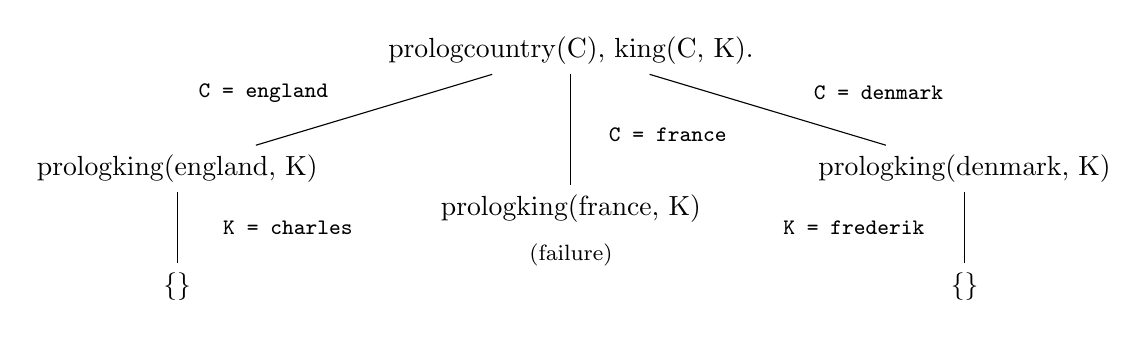
\begin{tikzpicture}
      \node (A) at (0,3) {\mintinline{prolog}{country(C), king(C, K).}};
      \node (B1) at (-5,1.5) {\mintinline{prolog}{king(england, K)}};
      \node (B2) at (0,1) {\mintinline{prolog}{king(france, K)}};
      \node (B3) at (5,1.5) {\mintinline{prolog}{king(denmark, K)}};
      \node (C1) at (-5,0) {\{\}};
      \node (C2) at (5,0) {\{\}};

      \draw (A) -- (B1) node [midway, xshift=-40, yshift=6] {\footnotesize \texttt{C = england}};
      \draw (A) -- (B2) node [midway, xshift=35, yshift=-2] {\footnotesize \texttt{C = france}};
      \draw (A) -- (B3) node [midway, xshift=40, yshift=6] {\footnotesize \texttt{C = denmark}};
      \draw (B1) -- (C1) node [midway, xshift=40] {\footnotesize \texttt{K = charles}};
      \draw (B3) -- (C2) node [midway, xshift=-40] {\footnotesize \texttt{K = frederik}};

      \node (D) at (0,0.4) {\footnotesize (failure)};
  \end{tikzpicture}
\end{center}
\caption{Search tree for the Prolog program}
\label{fig:prolog-search-tree}
\end{figure}

The tree is searched depth-first, left-to-right, with clauses selected in program order. Whenever there are multiple candidate clauses to resolve the current goal with, a \emph{choice point} is created, which stores the state of the execution at that point. If a dead end is reached, we \emph{backtrack} to the most recent choice point and try the next possible clause.

The \emph{empty clause} represents a contradiction, so deriving it means that a refutation of the negated query has been reached, and the current substitution can be returned as a solution. If all choice points have been exhausted without reaching the empty clause, no refutation can be found, so the query fails.

\subsection{Implementation}

\label{sec:preparation-implementation}

This subsection highlights some of the key decisions that must be made when building a Prolog implementation.

\paragraph{Unification} There are two common ways of implementing the unification subroutine, their signatures depicted in Figure \ref{fig:unification-impl} in Rust syntax. The first of these does not mutate the terms, instead returning an object representing their most general unifier, or failing, which I call \emph{substitution-based}. This is the approach taken by Tau Prolog \cite{riazaTauPrologProlog2024}. The second approach directly manipulates the term representations themselves to make them identical, or fails, as in the Warren Abstract Machine (WAM) \cite{warrenAbstractPrologInstruction1983}, which I call \emph{mutation-based}.

\begin{figure}[H]
\centering
\begin{minted}{rust}
fn unify1(a: &Term, b: &Term) -> Option<Substitution>;
fn unify2(a: &mut Term, b: &mut Term) -> Option<()>;
\end{minted}
\caption{Two styles of unification}
\label{fig:unification-impl}
\end{figure}

In a \emph{structure-copying} implementation, whenever a clause in the program is resolved with a goal, the terms representing that clause are copied and the variables in the copy bound according to the unifier. A \emph{structure-sharing} implementation recognises that different instances of the same term differ only in their variable bindings, so shares a \emph{prototype} between them, representing the individual instances as \emph{molecules} that store the variable bindings. Unification is more efficient with the former approach, but the latter can be more memory-efficient \cite{linewtermrepresentation1998}. These two representations are illustrated in Figure \ref{fig:term-representations}.

\begin{figure}[H]
\centering
\begin{subfigure}{.5\textwidth}
\centering
\begin{tikzpicture}
  \node (f) at (0,0) {$f$};
  \node (x) at (-1,-1) {$X$};
  \node (g) at (1,-1) {$g$};
  \node (4) at (-1,-2) {4};
  \node (3) at (0,-2) {3};
  \node (y) at (2,-2) {$Y$};
  \node (5) at (2,-3) {5};

  \draw[->] (f) -- (x);
  \draw[->] (f) -- (g);
  \draw[->] (x) -- (4) [dashed];
  \draw[->] (g) -- (3);
  \draw[->] (g) -- (y);
  \draw[->] (y) -- (5) [dashed];
\end{tikzpicture}
\caption{Structure-copying representation}
\end{subfigure}%
\begin{subfigure}{.5\textwidth}
\centering
\begin{tikzpicture}[triple/.style={draw, anchor=text, rectangle split, rectangle split horizontal, rectangle split parts=3}]
  \node (f) at (0,0) {$f$};
  \node (0) at (-1,-1) {$\langle 0 \rangle$};
  \node (g) at (1,-1) {$g$};
  \node (3) at (0,-2) {3};
  \node (1) at (2,-2) {$\langle 1 \rangle$};

  \node[triple] (b) at (3,-1) {$\bullet$ \nodepart{second} 4 \nodepart{third} 5};
  \node at (0,-2.75) {};

  \draw[->] (f) -- (x);
  \draw[->] (f) -- (g);
  \draw[->] (g) -- (3);
  \draw[->] (g) -- (y);

  \draw[->] (3.1,-0.92) to [out=180,in=0] (f);
\end{tikzpicture}
\caption{Structure-sharing representation}
\end{subfigure}
\caption{Representation of the term \texttt{f(X, g(Y))} with substitution $\{X \to 4, Y \to 5\}$}
\label{fig:term-representations}
\end{figure}

\paragraph{Variable Representation} Variables in Prolog are commonly represented as pointers to the term they are bound to, often with a mutation-based implementation. Unbound variables may be represented by a pointer to themselves, as in the WAM, or by a null pointer. Another approach, taken by Tau Prolog, is to assign an identifier to each variable upon creation, and store the bindings in a separate substitution data structure, which is more amenable to the substitution-based implementation.

\paragraph{Backtracking} When backtracking, variables that have been bound since the last choice point must be reset (unbound). This is often achieved by maintaining a stack called the \emph{trail}, which records variable bindings.

\paragraph{Memory Layout} There are several conceptually distinct areas of memory that a Prolog implementation often manages. These include

\begin{itemize}
\item the \emph{code area}, which stores the clauses of the program or the compiled instructions,
\item the \emph{local stack}, similar to the stack of a traditional programming language, which stores stack frames containing local terms (those certain not to be used outside the procedure) and return addresses,
\item the \emph{global stack} or \emph{heap}, which stores global terms (those that are not local),
\item the \emph{control stack}, which stores choice points, and
\item the \emph{trail}, which records variable bindings to be undone on backtracking.
\end{itemize}

Certain Prolog implementations combine some of these areas. For example, the WAM does not use a separate control stack, preferring to store choice points on the local stack. Tarau's ``hitchhiker'' virtual machine stores code on the heap rather than in a separate code area, as its encoding of instructions is the same as that of terms \cite{tarauHitchhikersGuideReinventing2018}. Li's Logic Virtual Machine (LVM) combines the stack and the heap into a single memory area to improve locality, which is managed by a garbage collector \cite{liEfficientMemoryManagement2000}.

\paragraph{Last-Call Optimisation (LCO)} The last predicate in the body of a clause can re-use the stack frame of its caller, and not create a choice point, if the clause is \emph{determinate}. That is, if the failure of the last predicate in the body implies the failure of the entire clause. Last-call optimisation enables programs like in Figure \ref{fig:lco} to run in constant stack space.

\begin{figure}[H]
\begin{center}
\begin{minted}{prolog}
len(L, N) :- len_acc(L, 0, N).
len_acc([], N, N).
len_acc([_|T], A, N) :- A1 is A + 1, len_acc(T, A1, N).
\end{minted}
\end{center}
\caption{A program to compute the length of a list in constant stack space}
\label{fig:lco}
\end{figure}

\section{Prolog Garbage Collection}

\label{sec:prolog-gc}

When backtracking to a choice point, any terms that were created since that choice point can be deallocated. This can be achieved by storing pointers to the top of the stack and the heap at each choice point, and truncating the stack and heap to these pointers when backtracking. This is known as \emph{instant reclaiming} \cite{bekkersDynamicMemoryManagement1992}.

However, instant reclaiming is insufficient for \emph{iterative} Prolog programs, that is, those which never backtrack. Consider the (contrived) program shown in Figure \ref{fig:iterative}, which sums the first $N$ natural numbers in constant stack space with LCO.

\begin{figure}[H]
\begin{center}
\begin{minted}{prolog}
sum(N, S) :- sum_acc(N, acc(0), S).
sum_acc(0, acc(N), N).
sum_acc(N, acc(A), S) :-
  N1 is N - 1,
  A1 is A + N,
  sum_acc(N1, acc(A1), S).
\end{minted}
\end{center}
\caption{A Prolog program that uses constant stack space but linear heap space}
\label{fig:iterative}
\end{figure}

By wrapping the accumulator in a functor \texttt{acc}, we force the Prolog implementation to allocate it, at each iteration, on the heap instead of the stack. Since heap memory is only reclaimed when backtracking, and this program never backtracks, the heap grows linearly with $N$.

To ensure programs like this do not run out of memory, many Prolog implementation use a \emph{garbage collector} to reclaim memory that is no longer reachable. This section gives an overview of garbage collection.

\subsection{Mark-and-Sweep}

\label{sec:prep-mark-and-sweep}

\emph{Mark-and-sweep} garbage collection operates in two phases. The \emph{root set} contains pointers to objects that are live, which are recursively followed to mark all reachable objects. Then, the heap is traversed again, and any unmarked objects are deallocated, often by \emph{compacting} the heap to remove the gaps left by deallocated objects.

Warren applied this algorithm to Prolog, using the local stack as the root set \cite{warrenImplementingPrologCompiling1977}. He emphasised, however, that due to the high cost of running the algorithm, it should only be run when necessary (i.e. when the heap is full), and that compile-time classification of variables into locals and globals (to minimise heap usage) is crucial for performance.

\subsection{Generational Garbage Collection}

\label{sec:generational-gc}

\emph{Generational garbage collection} attempts to mitigate the high performance cost of garbage collecting the entire heap by observing that most objects die young. This is called the \emph{generational hypothesis}.

The heap is divided into \emph{generations}, often two: the \emph{young generation}, where new objects are allocated, and the \emph{old generation}, where objects that survive a collection are promoted. The young generation is collected with frequent \emph{minor} collections, while infrequent \emph{major} collections cover the entire heap.

One complication with this approach is the existence of pointers from the old generation to the young generation. These must be considered part of the root set during a minor collection, so must be tracked by the garbage collector. Fortunately, in Prolog, there is already a mechanism for tracking pointers: the trail. Including the trail in the root set is sufficient to ensure that all reachable objects are marked, and that all pointers are correctly updated, without scanning the entire heap \cite{bekkersDynamicMemoryManagement1992}.

\section{Web Development with WebAssembly}

\label{sec:webdev}

For many years, the platform on which applications would run was the operating system (OS), executing native code but delegating to the OS via system calls for privileged functionality such as I/O. I call these applications \emph{native}. However, this requires applications to be built separately for different OSes and architectures, manually installed, and trusted.

For these reasons, more and more modern applications are delivered through the browser. I call these applications \emph{browser-based} or \emph{web applications}. Initially only for accessing information, the browser is now the platform on which word processors like Google Docs, videoconferencing applications like Teams, and even development environments like VSCode are built. These applications are written in a higher-level language like JavaScript, interpreted by the browser's JavaScript engine, with the browser providing built-in functions to access lower-level functionality, e.g. I/O. In this model, the browser is the only application that needs to be manually installed and trusted by the user.

Figure \ref{fig:web-platform} highlights the difference between native and web applications.

\begin{figure}[H]
\centering
\begin{subfigure}{0.5\textwidth}
  \centering
  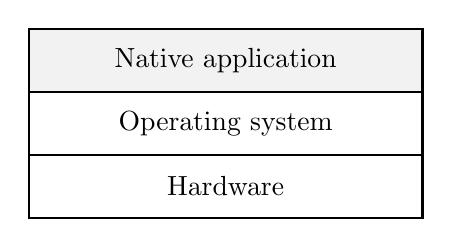
\begin{tikzpicture}[yscale=0.8]
    \fill[thick, black!5] (0,2) rectangle (5,3);
    \draw[thick] (0,0) rectangle (5,1);
    \draw[thick] (0,1) rectangle (5,2);
    \draw[thick] (0,2) rectangle (5,3);
    \node at (2.5,0.5) {Hardware};
    \node at (2.5,1.5) {Operating system};
    \node at (2.5,2.5) {Native application};
  \end{tikzpicture}
\caption{Native application}
\end{subfigure}%
\begin{subfigure}{0.5\textwidth}
  \centering
  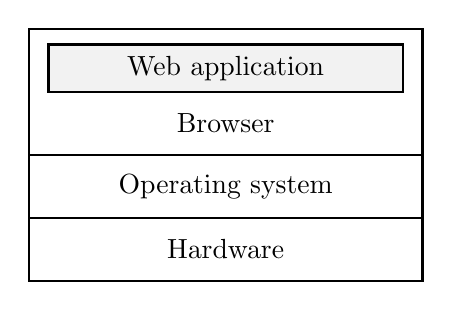
\begin{tikzpicture}[yscale=0.8]
    \fill[thick, black!5] (0.25,3) rectangle (4.75,3.75);
    \draw[thick] (0,0) rectangle (5,1);
    \draw[thick] (0,1) rectangle (5,2);
    \draw[thick] (0,2) rectangle (5,4);
    \draw[thick] (0.25,3) rectangle (4.75,3.75);
    \node at (2.5,0.5) {Hardware};
    \node at (2.5,1.5) {Operating system};
    \node at (2.5,2.5) {Browser};
    \node at (2.5,3.375) {Web application};
  \end{tikzpicture}
\caption{Web application}
\end{subfigure}
\caption{Native and web applications}
\label{fig:web-platform}
\end{figure}
\vspace*{-2em}

\subsection{Why WebAssembly?}

JavaScript has been the de facto language for web development since its introduction in 1995. Originally designed to bring interactivity to web pages, and famously built in 10 days, JavaScript has been continuously extended to become the world's most widely used programming language \cite{wirfs-brockJavaScriptfirst202020a}.

As web applications have increased in complexity, the consequences of JavaScript's complicated history have become more apparent. Being a high-level interpreted language, JavaScript is not well-suited for computationally intensive tasks. Similarly, its poor design as a language, for example its lack of static typing, makes large codebases difficult to maintain \cite{ocarizajr.JavaScriptErrorsWild2011, biermanUnderstandingTypeScript2014}.

For these reasons, supporting other programming languages on the Web has been a much discussed topic. Early proprietary attempts, such as Java applets, ActiveX, and Flash, have all since been deprecated due to security concerns\footnote{Early attempts to support other programming languages on the Web allowed native code to be directly embedded into the web page, which proved very difficult to sufficiently ``sandbox''.}. More recently, Emscripten has been used to compile C and C++ code to a subset of JavaScript called asm.js, designed to be easily optimised by the JIT compilers of JavaScript engines \cite{zakaiEmscriptenLLVMtoJavaScriptcompiler2011}. While this approach mitigates the security concerns of the previous technologies, it remains inherently limited by the performance of JavaScript.

WebAssembly was introduced in 2017 as a solution to the problem of running safe, fast, portable, low-level code on the Web \cite{haasBringingwebspeed2017}. It is a binary instruction format for a stack-based virtual machine that is designed to be a compilation target for high-level languages, and able to run in the browser at near-native speed.

\subsection{Memory Model}

\label{sec:wasm-memory-model}

The WebAssembly specification \cite{rossbergWebAssemblyCoreSpecification2022} is restrictive about how memory is accessed. The two areas of memory that are particularly relevant are the \emph{stack} and the \emph{linear memory}.

\paragraph{Stack}

A WebAssembly program executes as a \emph{stack machine}: operands of instructions are taken from the top of the stack, and results pushed back onto the stack. The stack also contains labels for control flow instructions, and \emph{activation frames} for function calls, which include local variables. Unlike the stack in a traditional language like C, the WebAssembly stack is not addressable; instead, local variables can only be referenced by their index from the stack pointer, meaning that stack-allocated variables cannot be passed to functions by reference. For example, in the C program below, the compiler must unintuitively allocate the local variable \texttt{x} in the linear memory, rather than on the stack, in order to pass it to the function \texttt{foo}.

\vspace*{-1em}

\begin{center}
\begin{minted}{c}
extern int foo(int*);
int main() {
  int x = 42;
  return foo(&x);
}
\end{minted}
\end{center}

\vspace*{-2em}

\paragraph{Linear Memory}

The main storage of a WebAssembly program is the \emph{linear memory}, or \emph{memory}, a contiguous array of bytes addressed by 32-bit pointers. These pointers are simply indices into the array. The memory is disjoint from the rest of the WebAssembly program. WebAssembly provides a \texttt{memory.grow} instruction to request that the host environment increases the size of the contiguous memory area (an operation like \texttt{realloc}), however, there is no way to free memory.

\subsection{Interface with JavaScript}

\label{sec:wasm-js-interface}

A key design goal of WebAssembly is to be \emph{language-independent}, thus the WebAssembly specification makes no mention of JavaScript. Instead, it is up to the \emph{host environment} (e.g. the browser) to define and implement the necessary APIs for WebAssembly to interact with the outside world.

\paragraph{Import and Export} WebAssembly modules can import and export functions to and from the host environment, allowing JavaScript code to call WebAssembly functions, and vice versa. However, only integers and floats can be passed between the two environments in this way.

\paragraph{Shared Memory} To enable more complex data structures to be shared, the browser exposes the WebAssembly module's linear memory to JavaScript as an array of bytes. This allows JavaScript code to serialise complex data structures into the linear memory, passing a pointer to the WebAssembly module, which can then access the data. WebAssembly functions can return complex data structures in the same way, illustrated in more detail in Appendix \ref{appendix:shared-memory}.

\section{Tools}

\label{sec:tools}

\paragraph{Rust}

Rust was chosen as the implementation language for the Prolog interpreter due to its strong support for WebAssembly and its focus on safety and performance. The officially-supported tool \texttt{wasm-bindgen} was used to facilitate interaction between Rust and JavaScript, alongside its companion tool \texttt{wasm-pack} for building and packaging the compiled WebAssembly module \cite{crichtonwasmbindgenhttpsgithubcom2014}.

\paragraph{Dependencies and Licensing}

Table \ref{tab:core-dependencies} lists the dependencies used in the implementation of the Prolog interpreter along with their licences, justifying the use of each. Table \ref{tab:web-dependencies} lists the dependencies used in the implementation of the browser-based development environment.

\begin{table}[H]
\centering
\begin{tabular}{lll}
\hline
\textbf{Name} & \textbf{Licence} & \textbf{Justification} \\
\hline
\texttt{wasm-bindgen}$^*$ & MIT/Apache-2.0 & Calls between Rust and JavaScript \\
\texttt{wasm-pack}$^*$ & MIT/Apache-2.0 & Build and package WebAssembly module \\
\texttt{js-sys}$^*$ & MIT/Apache-2.0 & Bindings to JavaScript APIs \\
Serde & MIT/Apache-2.0 & Serialise and deserialise data \\
\texttt{serde-wasm-bindgen} & MIT & Rust-JavaScript data type conversion \\
LALRPOP & MIT/Apache-2.0 & Generate the parser \\
\hline
\end{tabular}
\caption{Dependencies of the interpreter. Dependencies marked with a * are officially supported by the Rust WebAssembly Working Group.}
\label{tab:core-dependencies}
\end{table}

\begin{table}[H]
\centering
\begin{tabular}{lll}
\hline
\textbf{Name} & \textbf{Licence} & \textbf{Justification} \\
\hline
React & MIT & JavaScript framework for building UI \\
Next.js & MIT & Compile React components to static HTML \\
\texttt{react-simple-code-editor} & MIT & Code editor component \\
Prism & MIT & Syntax highlighting \\
Iconoir & MIT & Icons \\
\hline
\end{tabular}
\caption{Dependencies of the browser-based development environment}
\label{tab:web-dependencies}
\end{table}

\paragraph{Version Control}

Git was used for version control, with the repository hosted on GitHub. Each phase of development was carried out on a separate branch, with pull requests used to merge completed features into the \texttt{main} branch.

\paragraph{Continuous Integration} GitHub Actions, a GitHub service to automatically run code on repository events, was used for continuous integration, compiling and running the test suite on each push to the repository. GitHub's ``branch protection'' feature was employed to ensure that commits to the \texttt{main} branch could only be made through pull requests, and that all checks must pass before merging.

\paragraph{Deployment} The browser-based development environment was automatically built and deployed to Cloudflare Pages, a static website hosting service, on each push to the \texttt{main} branch, using GitHub Actions.

\section{Development Methodology}

\label{sec:dev-methodology}

The project was developed using a \emph{spiral} methodology \cite{boehmspiralmodelsoftware1986}, with development proceeding in a number of phases, each of which comprising requirements analysis, design, implementation, and testing. Evaluation in each phase involved quantitative comparison to existing Prolog implementations as described in Chapter 4, alongside qualitative comparison regarding feature completeness, which was then used to inform focus areas for the next phase.

The development phases were guided by the project proposal (Appendix \ref{appendix:proposal}), beginning with the implementation of a pure Prolog AST interpreter.

The project was tested using unit tests, integration tests, and manual testing. Unit tests were written for each phase to ensure its correctness before proceeding to the next phase. The benchmarking suite, described in Chapter 4, also served as a form of integration testing, as it was run in the browser and required the correct functioning of the system as a whole, with each benchmark program additionally acting as a test case. Manual testing was used to evaluate the browser-based development environment.

\section{Requirements Analysis}

\label{sec:requirements}

The core requirements are stated in the project proposal (Appendix \ref{appendix:proposal}) and are as follows:

\vspace*{-1em}

\begin{quote}
``The project will be deemed a success if I have written a Prolog interpreter in Rust, compiled it to WebAssembly, and executed it in the browser, as well as having compared its performance with existing solutions, including SWI-Prolog compiled to WASM and Tau Prolog.''
\end{quote}

\vspace*{-1em}

In the proposal, a number of extensions were also suggested. Following the background research outlined in this chapter, several of these were selected to be implemented as extensions. This research also highlighted the importance of a garbage collector in a practical Prolog implementation, so this was added as a further extension.

\begin{itemize}
\setlength{\itemsep}{0em}
\item \textbf{Cut and Extra-Logical Predicates}: Implementing the cut operator and some extra-logical predicates, which are key components of a full Prolog implementation.
\item \textbf{Development Environment}: A browser-based development environment to demonstrate and evaluate the interpreter.
\item \textbf{Garbage Collection}: A garbage collector to improve memory efficiency.
\item \textbf{JavaScript FFI}: An FFI to improve integration with the browser.
\end{itemize}

\section{Starting Point}

\label{sec:starting-point}

As detailed in the project proposal (Appendix \ref{appendix:proposal}), I began the project from scratch, with prior knowledge of Rust. I had little experience with Prolog, having only used it briefly in the Part IB course. No code was written before October 2024.